\documentclass{article}
\documentclass[12pt]{report}
\usepackage[utf8]{inputenc}
\usepackage[russian]{babel}
%\usepackage[14pt]{extsizes}
\usepackage{listings}
\usepackage{graphicx}
\usepackage{amsmath,amsfonts,amssymb,amsthm,mathtools} 
\pagestyle{empty}

% Настройка листинга кода:
\lstset{ %
language=assembly,                
basicstyle=\small\sffamily, % размер и начертание шрифта для подсветки кода
%numbers=left,               % где поставить нумерацию строк (слева\справа)
numberstyle=\tiny,           % размер шрифта для номеров строк
stepnumber=1,                   % размер шага между двумя номерами строк
numbersep=5pt,                % как далеко отстоят номера строк от подсвечиваемого кода
showspaces=false,            % показывать или нет пробелы специальными отступами
showstringspaces=false,      % показывать или нет пробелы в строках
showtabs=false,             % показывать или нет табуляцию в строках
frame=single,              % рисовать рамку вокруг кода
tabsize=2,                 % размер табуляции по умолчанию равен 2 пробелам
captionpos=t,              % позиция заголовка вверху [t] или внизу [b] 
breaklines=true,           % автоматически переносить строки (да\нет)
breakatwhitespace=false, % переносить строки только если есть пробел
escapeinside={\#*}{*)}   % если нужно добавить комментарии в коде
}

%\title{Лабораторная работа №1 (часть 1)}

\begin{document}

\section{Листинг прерывания int 8h: }
\begin{lstlisting}[label=some-code,caption=Листинг перывания int 8h]
Temp.lst			Sourcer	v5.10   18-Sep-20  12:16 pm   Page 1

020A:0746  E8 0070				call	sub_1			; (07B9)
020A:0749  06					push	es
020A:074A  1E					push	ds
020A:074B  50					push	ax
020A:074C  52					push	dx
020A:074D  B8 0040				mov	ax,40h
020A:0750  8E D8				mov	ds,ax
020A:0752  33 C0				xor	ax,ax		
020A:0754  8E C0				mov	es,ax
020A:0756  FF 06 006C			inc	word ptr ds:[6Ch]	
020A:075A  75 04				jnz	loc_1		
020A:075C  FF 06 006E			inc	word ptr ds:[6Eh]
020A:0760			loc_1:
020A:0760  83 3E 006E 18		cmp	word ptr ds:[6Eh],18h
020A:0765  75 15				jne	loc_2			
020A:0767  81 3E 006C 00B0		cmp	word ptr ds:[6Ch],0B0h	
020A:076D  75 0D				jne	loc_2			
020A:076F  A3 006E				mov	word ptr ds:[6Eh],ax	
020A:0772  A3 006C				mov	word ptr ds:[6Ch],ax	
020A:0775  C6 06 0070 01		mov	byte ptr ds:[70h],1
020A:077A  0C 08				or	al,8
020A:077C			loc_2:
020A:077C  50					push	ax
020A:077D  FE 0E 0040			dec	byte ptr ds:[40h]	
020A:0781  75 0B				jnz	loc_3		
020A:0783  80 26 003F F0		and	byte ptr ds:[3Fh],0F0h	
020A:0788  B0 0C				mov	al,0Ch
020A:078A  BA 03F2				mov	dx,3F2h
020A:078D  EE					out	dx,al		
020A:078E			loc_3:
020A:078E  58					pop	ax
020A:078F  F7 06 0314 0004		test	word ptr ds:[314h],4	 

020A:0795  75 0C				jnz	loc_4			
020A:0797  9F					lahf				
020A:0798  86 E0				xchg	ah,al
020A:079A  50					push	ax
020A:079B  26: FF 1E 0070			call	dword ptr es:[70h]
020A:07A0  EB 03				jmp	short loc_5
020A:07A2  90					nop
020A:07A3			loc_4:
020A:07A3  CD 1C				int	1Ch		
020A:07A5			loc_5:
020A:07A5  E8 0011				call	sub_1		
020A:07A8  B0 20				mov	al,20h		
020A:07AA  E6 20				out	20h,al			
										
020A:07AC  5A					pop	dx
020A:07AD  58					pop	ax
020A:07AE  1F					pop	ds
020A:07AF  07					pop	es
020A:07B0  E9 FE99				jmp	$-164h
020A:07B3  C4					db	0C4h
							                       
020A:07B4  C4 0E 93E9			les	cx,dword ptr ds:[93E9h]	

020A:07B8  FE					db	0FEh
\end{lstlisting}

\section{Схема алгоритма прерывания int 8h: }
\vspace{1em}
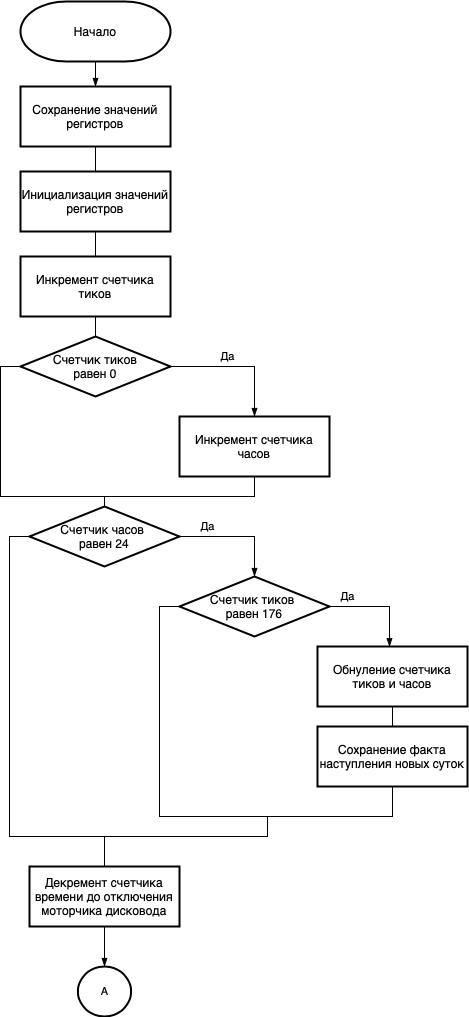
\includegraphics[width=0.60	\linewidth]{os1.png}
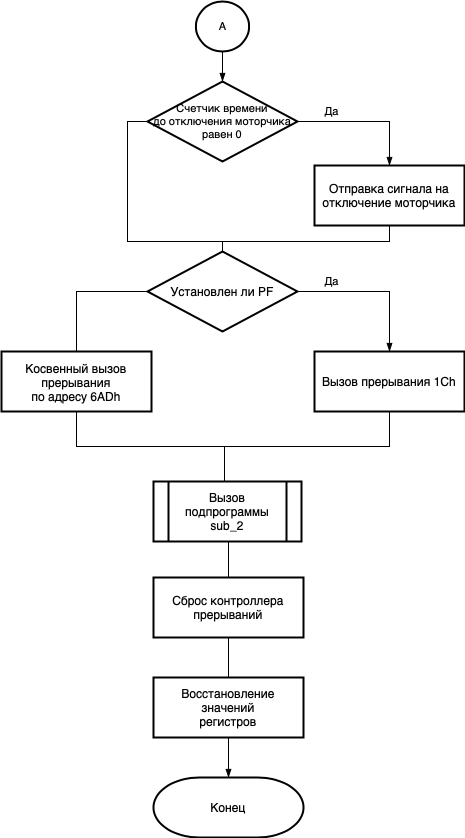
\includegraphics[width=0.60	\linewidth]{os12.png}
\vspace{2em}
\section{Листинг подпрограммы sub1: }
\begin{lstlisting}[label=some-code,caption=Листинг подпрограммы sub_1:]
				sub_1		proc	near
020A:07B9  1E					push	ds
020A:07BA  50					push	ax
020A:07BB  B8 0040				mov	ax,40h
020A:07BE  8E D8				mov	ds,ax
020A:07C0  9F					lahf			
020A:07C1  F7 06 0314 2400			test	word ptr ds:[314h],2400h	
020A:07C7  75 0C				jnz	loc_7			
020A:07C9  F0> 81 26 0314 FDFF	lock	and	word ptr ds:[314h],0FDFFh	
020A:07D0			loc_6:
020A:07D0  9E					sahf			
020A:07D1  58					pop	ax
020A:07D2  1F					pop	ds
020A:07D3  EB 03				jmp	short loc_8	
020A:07D5			loc_7:
020A:07D5  FA					cli				    
020A:07D6  EB F8				jmp	short loc_6	
020A:07D8			loc_8:
020A:07D8  C3					retn
				sub_1		endp
\end{lstlisting}



\section{Схема алгоритма обработки прерывания от системного таймера:}
\vspace{1em}
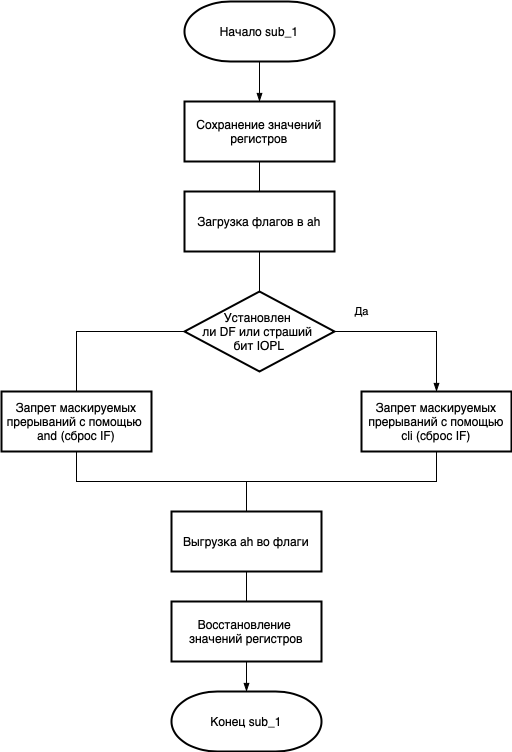
\includegraphics[width=0.90	\linewidth]{os2.png}

\vspace{1em}
\section{Функция обрабочика прерывания}
\vspace{1em}
\begin{itemize}
    \item Инкремент значения счетчика тиков;
    \item Контроль переполнения счетчика тиков (наступление нового дня);
    \item Декремент времени, оставшегося до выключения моторчика дисковода;
    \item Выключение моторчика дисковода, по истечению таймера;
    \item Вызов пользовательского прерывания 1Ch (IRET). С помощью которого можно совершать периодические действия;
\end{itemize}

\section{Вывод}
В данной лабораторной работе я научился получать адрес начала прерывания и листинг прерывания с помощью дизассемблирования участка кода. Проанализирвоал алгоритм работы прерывания int 8h. Это прерывание отвечает за изменение счётчика системного времени, управление контроллером дисковода с целью минимизировать времени работы моторчика дисковода, является способом периодического вызова пользовательского прерывания. 
\end{document}
